% *********************************************************************
% © 2016–2019 Jeremy Sylvestre
%
% Permission is granted to copy, distribute and/or modify this document
% under the terms of the GNU Free Documentation License, Version 1.3 or
% any later version published by the Free Software Foundation; with no
% Invariant Sections, no Front-Cover Texts, and no Back-Cover Texts. A
% copy of the license is included in the appendix entitled “GNU Free
% Documentation License” that appears in the output document of this
% PreTeXt source code. All trademarks™ are the registered® marks of
% their respective owners.
% 
% *********************************************************************
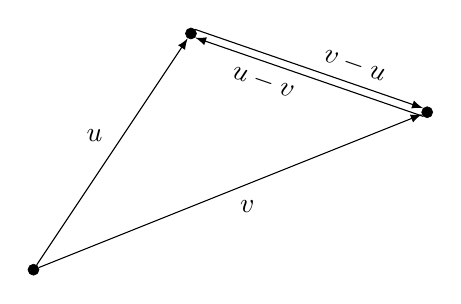
\begin{tikzpicture}[
	point/.style={circle,draw,very thin,fill,inner sep=0pt,minimum size=4pt},
	vector/.style={-latex},
]
	\node[point] at (0,0) (p) {};
	\node[point] at (2,3) (q) {};
	\node[point] at (5,2) (r) {};
	\draw[vector] (p) to node[above left] {$\uvec{u}$} (q);
	\draw[vector] (p) to node[below right] {$\uvec{v}$} (r);
	\draw[vector] (r.south west) to node[below left,sloped] {$\uvec{u}-\uvec{v}$} (q.south east);
	\draw[vector] (q.north east) to node[above right,sloped] {$\uvec{v}-\uvec{u}$} (r.north west);
\end{tikzpicture}
